\chapter{Conceptos previos}


\section{Machine Learning}

Se entiende como el campo de las ciencias de computación que en vez de enfocarse en el diseño de algoritmos explícitos, optan por el estudio de técnicas de aprendizaje. Este enfoque tiene un gran éxito en tareas computacionales donde no es factible diseñar un algoritmo de forma explícita. \cite{Programming_Massively} \\
En vez de averiguar las distintas reglas a seguir para llegar a una solución, esta alternativa permite simplemente suministrar ejemplos de lo que debería pasar en distintas situaciones, y dejar que la máquina aprenda y extraiga ella misma sus propias conclusiones. De esta forma, el procedimiento en aprendizaje supervisado consiste en 'entrenar' con una muestra de N ejemplos, extraer información de ellos, y posteriormente poder evaluar de forma 'correcta' (bajo un margen de error controlado) otra muestra de M ejemplos, siendo M \textgreater N. \cite{Learning_From_Data} \\
Este enfoque ha contribuido en el avance de áreas como reconocimiento de voz, visión por ordenador, procesamiento de lenguaje natural, etc.

\section{Componentes necesarios para el aprendizaje supervisado}

Datos de entrada X y de salida Y que el modelo empleará para aprender y tomar decisiones. Ambos se unen para formar un dataset de entradas-salidas D=\{($x_1, y_1$), ($x_2, y_2$), ..., ($x_N, y_N$)\}. Para que el aprendizaje sea posible, debe existir una función F: X $\rightarrow$ Y tal que $y_i$ = F($x_i$) para i$\in$\{1...N\}. De esta forma, en función del dataset D, el modelo tratará de encontrar una función G que aproxime F para dicho conjunto. Además, se suelen aplicar técnicas que permitan una mejor generalización del modelo, expandiendo las capacidades del mismo y permitiendo que su conocimiento pueda ser útil incluso fuera de la muestra de datos inicial. \cite{Learning_From_Data}

\section{División de datos en entrenamiento y test}

Para visualizar la generalización del modelo, el conjunto de datos D se suele dividir en 2 subconjuntos, (entrenamiento y test) de forma que se pueda estimar si realmente 'aprende' o solo memoriza.\\
Una vez realizada la división, se entrena el modelo con los datos del conjunto de entrenamiento. Cuando se termina el entrenamiento, se accede al conjunto test y se visualiza el rendimiento del modelo sobre el mismo. Como los datos de test no se emplearon en ningún momento, aportan una estimación sobre la generalización del modelo fuera de la muestra con la que se entrenó. 

\section{Tipos de aprendizaje}

\subsection{Aprendizaje Supervisado}

% \cite{Learning_From_Data} página 24

Es el que se empleará en este proyecto. 
Se caracteriza por la presencia de una etiqueta 'correcta' $y_i$ asociada a cada dato de entrada $x_i$. Posteriormente, la red empleará ambos valores para, a partir de $x_i$, tratar de deducir $y_i$. \cite{Learning_From_Data} \\
Aunque se trate de impedir, la existencia de ruido en los datos es inevitable, implicando que algunas etiquetas de Y=$\{y_1, y_2, ..., y_N\}$ puedan ser erróneas. \\
Este tipo de aprendizaje se divide a su vez en problemas de clasificación y regresión, centrándose en predecir etiquetas o valores numéricos, respectivamente.

\subsection{Aprendizaje No Supervisado}

En este tipo de aprendizaje los datos no contienen ninguna información respecto a Y. De esta forma, el conjunto de datos D se compone exclusivamente de valores X=$\{x_1, x_2, ..., x_N\}$. \cite{Learning_From_Data}

\subsection{Aprendizaje Por Refuerzo}

En este caso tampoco existe un $y_i$ 'correcto' asociado a cada $x_i$. En su lugar, se asocia a cada $x_i$ una etiqueta con un valor posible de $y_i$, además de una medida que indica como de bueno es el mismo. \cite{Learning_From_Data}


\section{Redes Neuronales Totalmente Conectadas}

\subsection{Neurona}

\begin{figure}[H]
	\centering
	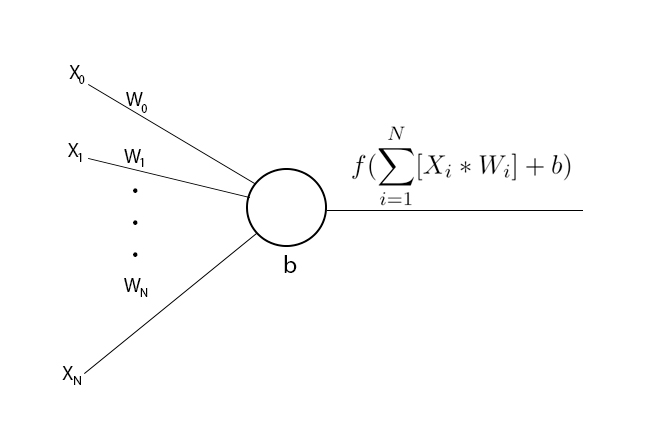
\includegraphics[scale=0.35]{imagenes/neurona.jpg}  
	\caption{Imagen de una neurona}
	\label{fig:neurona}
\end{figure}

Una neurona parte de una serie de datos de entrada X=\{$x_1$, $x_2$, ..., $x_N$\} tal que cada $x_i$$\in${X} se encuentra asociado a un peso $w_i\in{W}$. \\
Esta los emplea para realizar una suma ponderada y posteriormente añadir un sesgo b, además de aplicar una función de activación f sobre el resultado obtenido. 

\subsection{Estructura por capas}

\begin{figure}[H]
	\centering
	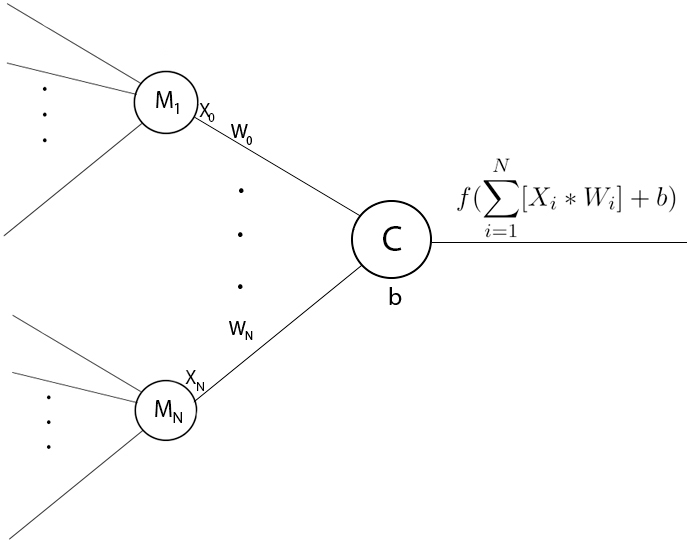
\includegraphics[scale=0.35]{imagenes/capa_neuronas.jpg}  
	\caption{Imagen de una capa de neuronas}
	\label{fig:capa_neuronas}
\end{figure}

Las neuronas se suelen agrupas por capas, de tal forma que la salida de una compone la entrada de la siguiente, formando así modelos más sofisticados.

\subsection{Funciones de activación}

\subsubsection{ReLU}

\begin{gather}
	ReLU(x) = max(0, x)
\end{gather}

\begin{figure}[H]
	\centering
	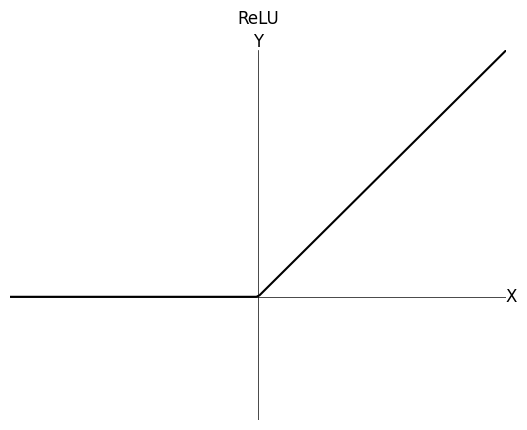
\includegraphics[scale=0.45]{imagenes/ReLU.jpg}  
	\caption{Imagen de la función de activación ReLU}
	\label{fig:ReLU}
\end{figure}

A cambio de un bajo coste computacional, aporta no linealidad a la neurona, permitiendo a esta aprender funciones de mayor complejidad. \\
Como su gradiente es 0 o 1, evita una reducción excesiva del mismo para valores positivos, mitigando así el problema del desvanecimiento del gradiente, caracterizado por la presencia de gradientes muy pequeños en backpropagation y provocar un aprendizaje lento. \cite{ReLU}

\subsubsection{Sigmoide}

\begin{gather}
	sigmoide(x) = \frac{1}{1+e^{-x}}
\end{gather}

\begin{figure}[H]
	\centering
	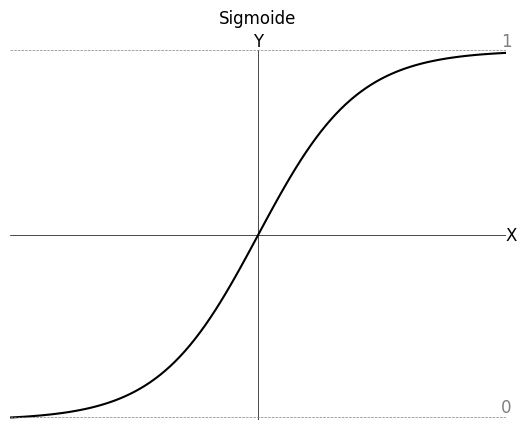
\includegraphics[scale=0.45]{imagenes/sigmoide.jpg}  
	\caption{Imagen de la función de activación Sigmoide}
	\label{fig:Sigmoide}
\end{figure}

Se trata de una función interesante en el ámbito de la clasificación binaria, pues se caracteriza por transformar un valor de entrada en una salida comprendida en el rango [0-1]. \\
Aunque sea monótona creciente y diferenciable en todos los puntos, tiende a saturarse con valores extremos (positivos o negativos). Por tanto, su aplicación dependerá del caso concreto a tratar. \cite{Sigmoide}

\subsubsection{SoftMax}

\begin{figure}[H]
	\centering
	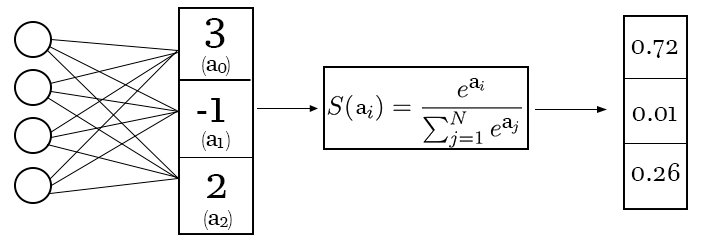
\includegraphics[scale=0.35]{imagenes/softmax.jpg}  
	\caption{Imagen de la función de activación SoftMax}
	\label{fig:SoftMax}
\end{figure}

Para n entradas, produce n salidas con valores en el rango [0-1] que mantienen la proporción de entrada y cuya suma es 1. Por tanto, se pueden interpretar como la probabilidad de pertenencia a cada clase, siendo especialmente útil en clasificación multiclase. \cite{SoftMax_MLM} \\
\subsection{One-hot encoding}

\subsection{Función de error o pérdida}

\subsubsection{Entropía Cruzada}

\begin{gather}
	E(y, \hat{y}) = - \sum_{i=1}^{H}  [y_i * log( \hat{y}_i)]
	\label{loss_func_softmax}
\end{gather}

Es una métrica empleada en aprendizaje automático para medir qué tan bien se desempeña un modelo de clasificación. La pérdida o error se mide como un valor en el rango [0-1], siendo 0 un modelo perfecto y 1 otro totalmente erróneo. \cite{Cross_entropy}

H es el número de clases al que puede pertenecer cada dato de entrada $x_i \in X$.


% https://medium.com/mlearning-ai/understanding-loss-functions-for-classification-81c19ee72c2a

\subsubsection{Sigmoid Cross Entropy Loss}
Es un caso particular de entropía cruzada caracterizado por la presencia de un número de clases igual a 2.

\begin{gather}
	E(x) = - \frac{1}{N} \sum_{i=1}^{N}  [y_i * log( \hat{y}_i) + (1-y_i)*log(1-\hat{y_i})]
	\label{loss_func}
\end{gather}

y = etiqueta real \\
$\hat{y}$ = predicción 

\subsection{Descenso del gradiente}

\begin{figure}[H]
	\centering
	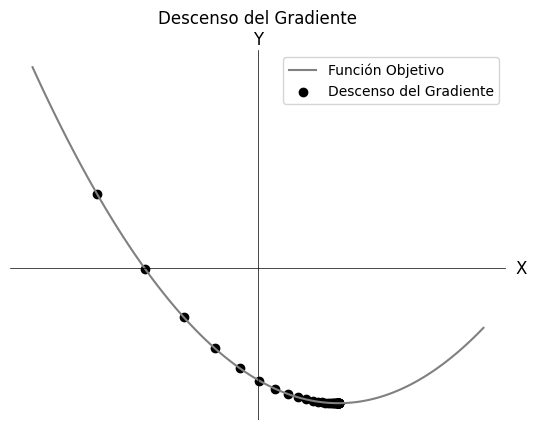
\includegraphics[scale=0.4]{imagenes/sgd.jpg}  
	\caption{Ejemplo de funcionamiento del descenso del gradiente}
	\label{fig:SGD}
\end{figure}

Es un método de optimización iterativo que busca el mínimo local en una función diferenciable. En la figura \ref{fig:SGD} se muestra un ejemplo del mismo, donde cada punto representa una iteración del algoritmo. \\
Su nombre viene del término 'gradiente', siendo este una generalización multivariable de la derivada y denominado por el símbolo $\nabla$. Para una función f y un punto p, este indica la dirección del máximo incremento en la misma. El descenso del gradiente usa esta información para, una vez obtenido el gradiente, desplazarse en dirección contraria, es decir, en dirección del mínimo. Además, la distancia que se recorre en cada iteración viene dada por un hiperparámetro denominado ``learning rate'' o $\alpha$. \cite{SGD_1} \cite{Gradiente} \cite{SGD_2} \\


\subsubsection{Entrenamiento}
De esta forma, el procedimiento para entrenar una red neuronal consiste en, para una entrada $x_i$ y una etiqueta asociada $y_i$, emplear $x_i$ para producir una predicción $\hat{y}_i$ (\textbf{ForwardPropagation} o Propagación hacia delante) que posteriormente se podrá comparar con $y_i$ mediante una función de error H(x) y obtener una medida de lo buena o mala que fue la misma. Una vez obtenido dicho ``error'', se aplica el algoritmo del descenso del gradiente para cada parámetro de la red (\textbf{BackPropagation} o retropropagacion). \cite{Cross_entropy} \\

\begin{gather}
	W_{t+1} = W_{t} - \alpha * \frac{\partial H(x)}{\partial W_{t}} 
	\label{act_pesos}
\end{gather}

\begin{gather}
	b_{t+1} = b_{t} - \alpha * \frac{\partial H(x)}{\partial b_{t}}
	\label{act_bias}
\end{gather}


Así, se actualizarán los parámetros de la red neuronal según las fórmulas \ref{act_pesos} y \ref{act_bias}. En ellas, $W_t$ y $b_t$ indican los valores del peso W y bias b en el instante o iteración t, de la misma forma que $W_{t+1}$ y $b_{t+1}$ representan los valores de los mismos en el instante t+1. \cite{SGD_act_params}

\subsection{Inicialización de pesos y sesgos}

\subsubsection{Inicialización de pesos}
Como función de activación se empleará ReLU. Por tanto, tal y como se indica en la bibliografía, se inicializan los pesos mediante la ``inicialización He'' o ``inicialización Kaiming He''. Esta consiste en, para un peso $w$, inicializarlo según una distribución gaussiana con una media de 0.0 y una desviación típica de $\sqrt{\frac{2}{N\_in}}$, siendo $N\_in$ el número de neuronas en la capa de entrada.
 \cite{ini_He} \cite{ini_He_2} \cite{ini_He_code}.

\subsubsection{Inicialización de sesgos}

De la misma forma, se sigue la bilbiografía y los sesgos se inicializarán a 0.0 . \cite{ini_bias} \cite{ini_bias_2}

\subsection{Tipos de codificaciones}

En el campo de machine learning existen varios tipos de codificaciones. De esta forma, para codificar 3 clases distintas se podrían codificar o bien mediante \{1, 2, 3\} (codificación de etiquetas), o mediante \{100, 010, 001\} (codificación one-hot), por ejemplo. En este proyecto se empleará la codificación one-hot, pues aporta unas ventajas que se contemplarán con detalle en secciones posteriores.

\subsection{Propagación hacia delante con softmax}

Suponemos que para un $x_i$ dado, se obtiene S($\hat{y}$) = [ S($\hat{y}_1)$, S($\hat{y}_2)$, S($\hat{y}_3)$ ] = [0.04, 0.7, 0.26 ] \\
Para dicho $x_i$, $y_i$ = [0, 0, 1] \\
En este caso, el modelo cree que $x_i$ pertenece a la clase 2 (0.7 es el mayor número del vector S($\hat{y})$). Sin embargo, $y_i$ indica que $x_i$ pertenece a la clase 3. \\

Se calcula el error de entropía cruzada: \\

\begin{gather}
	 E(y, S(\hat{y})) = - (0*log(0.04) + 0*log(0.7) + 1*log(0.26)) \\
	 E(y, S(\hat{y})) = -log(0.26) = 0.585
\end{gather}

\cite{Cross_entropy_backprop}

\section{Redes Neuronales Convolucionales}

\subsection{Capa convolucional}

\subsubsection{Componentes}

\begin{figure}[H]
	\centering
	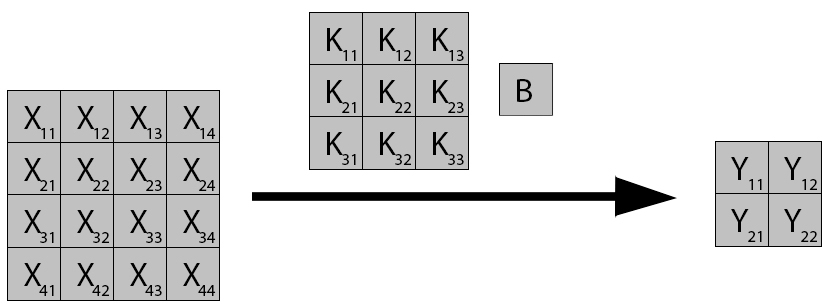
\includegraphics[scale=0.35]{imagenes/conv_nombres.jpg}  
	\caption{Componentes en una capa convolucional}
	\label{fig:Componentes_convolucion}
\end{figure}

Una capa convolucional parte de un volumen de entrada X, un kernel de filtros K y un sesgo B para, mediante una convolución, obtener un volumen de salida Y.

\subsubsection{Propagación hacia delante}

\begin{figure}[H]
	\centering
	\begin{subfigure}{.5\textwidth}
		\hspace{-10mm}
		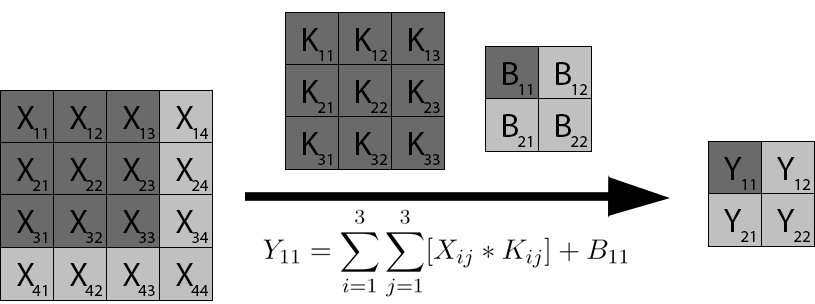
\includegraphics[width=1.2\linewidth]{imagenes/conv_1.jpg}  
		\caption{Cálculo $Y_{11}$}
	\end{subfigure}%
	\begin{subfigure}{.5\textwidth}
		\hspace{10mm}
		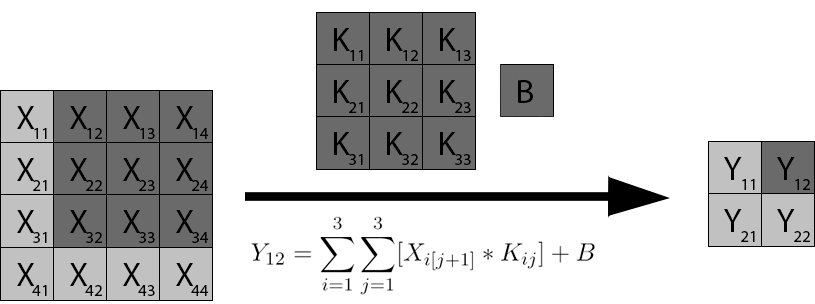
\includegraphics[width=1.2\linewidth]{imagenes/conv_2.jpg}  
		\caption{Cálculo $Y_{12}$}
	\end{subfigure}
	
	\vspace{5mm}
	\begin{subfigure}{.5\textwidth}
		\hspace{-10mm}
		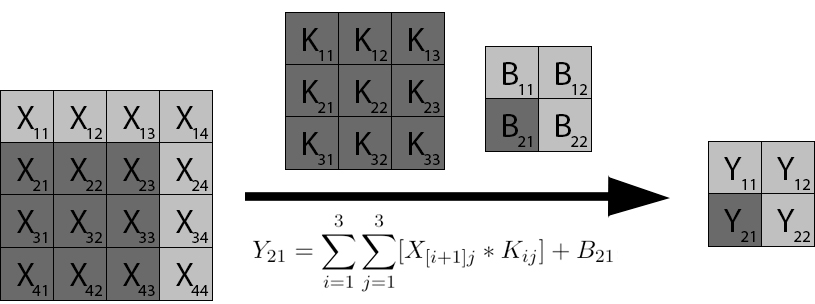
\includegraphics[width=1.2\linewidth]{imagenes/conv_3.jpg}  
		\caption{Cálculo $Y_{21}$}
	\end{subfigure}%
	\begin{subfigure}{.5\textwidth}
		\hspace{10mm}
		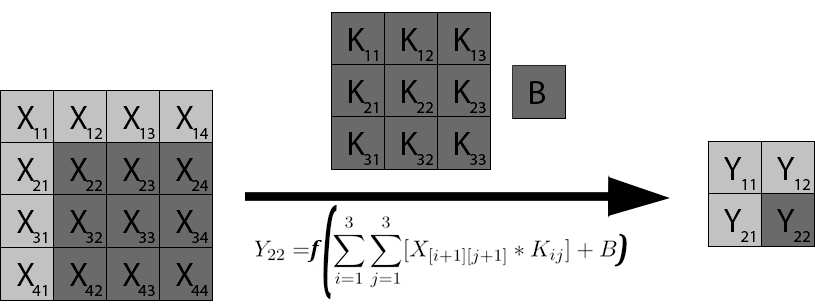
\includegraphics[width=1.2\linewidth]{imagenes/conv_4.jpg}  
		\caption{Cálculo $Y_{22}$}
	\end{subfigure}
	\caption{Propagación hacia delante en una capa convolucional}
	\label{fig:forward_prop_convolucional}
\end{figure}

\begin{gather}
	 Y_{11} = \sum_{i=1}^{3} \sum_{j=1}^{3} [X_{ij}*K_{ij}] + B_{11}
\end{gather}



\subsection{Capa de agrupación o pooling}

\subsubsection{Componentes}

\subsubsection{Propagación hacia delante}

\subsection{Capa de aplanado}

\subsubsection{Propagación hacia delante}
